In this section we describe the kinematics, acceptances, and projected
uncertainties. The projections have been made for 50 days of running with a
luminosity of $10^{37}$ cm$^{-2}$s$^{-1}$ on a 15 cm long liquid hydrogen
target. Only statistical uncertainties are shown. To scale to 100 days of
running, simply reduce the error bar by a factor of 0.7.

The projections are binned in three  kinematic variables: the virtuality
of the final-state photon $Q^{\prime 2} = M_{e^+e^-}^2$, the four-momentum
transfer to the nucleon $t$, and the skewness of the reaction $\eta$. The
angular distribution of the decay-lepton pair is evaluated in each bin, for
instance as a moment of the weighted cross section, using the lepton
center-of-mass angles shown in Fig.~\ref{fig:Angle}. To avoid confusion with
the lab angles, we will in this section excplicitly call these angles
$\theta_{CM}$ and $\varphi_{CM}$.


\subsection{Acceptance}
\label{sec:acc}

The selection of exclusive $e^+e^-p$ events was discussed in
Sect.~\ref{sec:tcs_selection}. Since the TCS cross section will not be
measured separately but in combination with the larger BH cross section with
which it interferes, the rate estimates for TCS were based on the BH cross
section as given in Ref.~\cite{vadim}. The resulting event distributions, 
illustrating the SoLID acceptance, are shown in Figs.~\ref{fig:t_Q2_etabin}
through \ref{fig:theta_phi_CM_Q2bin}. The first two figures show the
acceptance in six bins of $\eta$, and the last two in three bins of
$Q^{\prime 2}$. The former binning is suited for measuring the
$Q^{\prime 2}$-dependence in narrow bins of $\eta$ to study factorization
and higher-twist effects, while the latter is better for looking at the
$\eta$-dependence in wider bins of $Q^{\prime 2}$, primarily in order to
understand the impact of NLO corrections.

Fig.~\ref{fig:t_Q2_etabin} shows how the accessible range in $Q^{\prime 2}$
grows at higher values of $\eta$. It also shows how the $|t|$-coverage
shifts to higher values as $\eta$ increases.
The choice of six bins in $\eta$ is arbitrary. It is based on a desire to
to make an initial study of the $Q^{\prime 2}$-dependence in sufficiently
narrow bins in $\eta$ the interpretation will not be complicated by 
large NLO corrections. In actual  analysis, the $Q^{\prime 2}$-dependence
will also be investigated in wide $\eta$ bins. The widths of the six bins
shown have been chosen to equalize statistics in the range $0.1<\eta<0.4$
that can be covered in SoLID.
Fig.~\ref{fig:theta_phi_CM_etabin} shows the event distributions in the
$\theta_{CM}$ vs. $\varphi_{CM}$ plane for the same six bins in $\eta$.
The shape of the acceptance in the lepton CM-angles is governed by three
factors: the ``hole'' in the forward detector around the beam line, the
limit of the large-angle acceptance, and the gap between the large-angle
and forward-angle detectors in SoLID. 
The first two define the general overall shape of the distribution, while
the gap leads to a depletion of events in the middle of the band.

\begin{figure}[t]
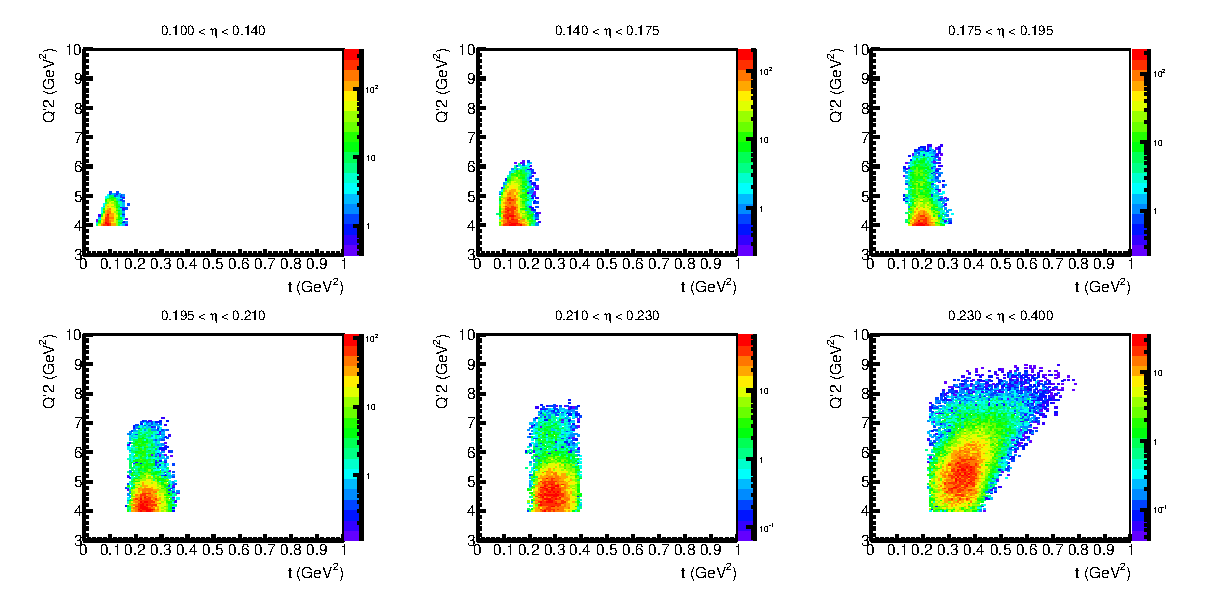
\includegraphics[scale=0.8]{t_Q2_etabin.eps}
\caption{\small{BH event distribution, in TCS kinematics, showing the SoLID
acceptance for exclusive $e^+e^-p$ production and showing the accessible
range in $Q^{\prime 2}$ and $|t|$ for six bins of $\eta$.}}
\label{fig:t_Q2_etabin}
\end{figure}

\begin{figure}[t]
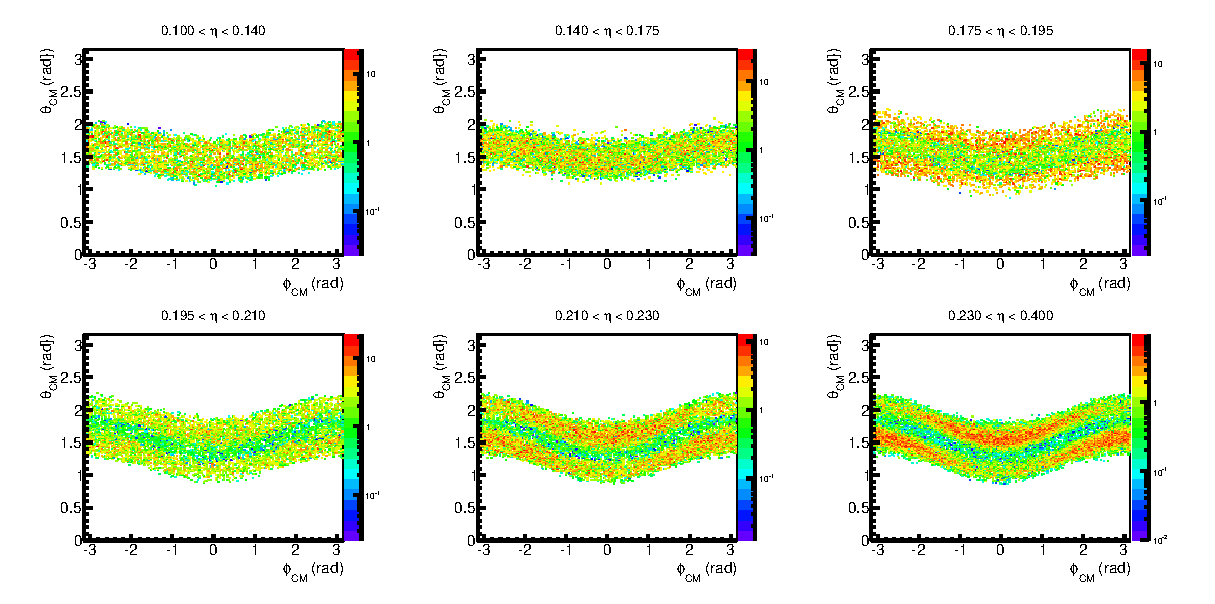
\includegraphics[scale=0.8]{theta_phi_CM_etabin.eps}
\caption{\small{BH event distribution, in TCS kinematics, showing the SoLID
acceptance for exclusive $e^+e^-p$ production and showing the accessible range
in $\theta_{CM}$ and $\varphi_{CM}$ for six bins of $\eta$.}}
\label{fig:theta_phi_CM_etabin}
\end{figure}

Once the $Q^{\prime 2}$-scaling is understood, studying the NLO corrections
through the $\eta$-dependence will not require very narrow bins in
$Q^{\prime 2}$. Fig.~\ref{fig:t_eta_Q2bin} shows the distribution of events
in $\eta$ and $|t|$ in two bins of $Q^{\prime 2}$.
Fig.~\ref{fig:theta_phi_CM_Q2bin} shows the corresponding distributions in
the $\theta_{CM}$ vs. $\varphi_{CM}$ plane.

\begin{figure}[t]
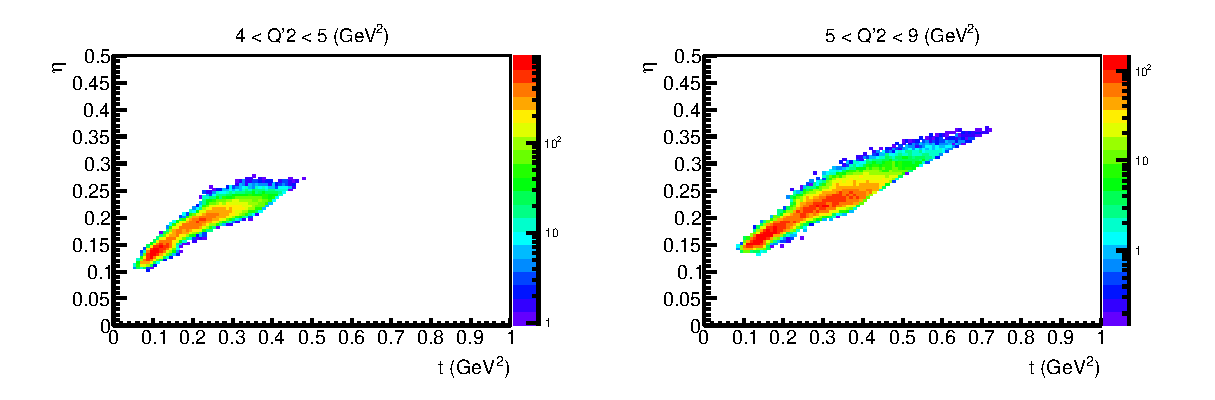
\includegraphics[scale=0.7]{t_eta_Q2bin.eps}
\caption{\small{BH event distribution, in TCS kinematics, showing the SoLID
acceptance for exclusive $e^+e^-p$ production and showing the accessible
range in $\eta$ and $|t|$ for two bins in $Q^{\prime 2}$.}}
\label{fig:t_eta_Q2bin}
\end{figure}

\begin{figure}[t]
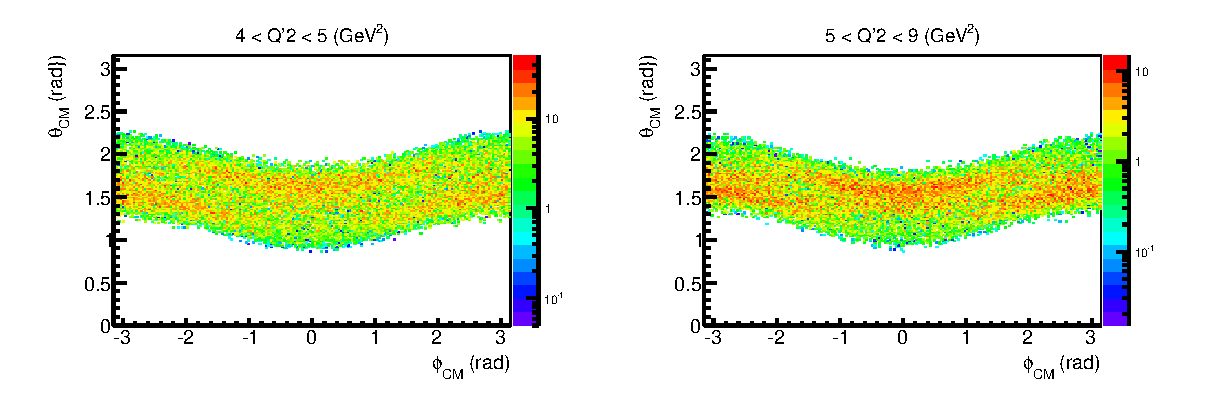
\includegraphics[scale=0.7]{theta_phi_CM_Q2bin.eps}
\caption{\small{BH event distribution, in TCS kinematics, showing the SoLID
acceptance for exclusive $e^+e^-p$ production and showing the accessible
range $\theta_{CM}$ and $\varphi_{CM}$ for tho bins of $Q^{\prime 2}$.}}
\label{fig:theta_phi_CM_Q2bin}
\end{figure}


\subsection{Projections}
\label{sec:tcsrate}

The results from the TCS analysis will come in the form of the measured
differential cross section as well as cosine and sine moments of the weighted
cross section. The cross section measurement will constrain global fits of
Compton form factors (CFFs), and could be used for extraction of helicity
amplitudes, which are related to the CFFs through Eq.~(\ref{eq:M}), by fitting
the data in the SoLID $\theta_{CM}$-$\varphi_{CM}$ acceptance.
The cosine and sine moments are also directly related to the helicity
amplitudes (and hence CFFs and GPDs). A comparison of the moments, evaluated
within the SoLID acceptance, imposes strong constraints on GPD models, and in
particular for the real part of the amplitude. 

The experimental sensitivity of the proposed measurement is easiest to
evaluate through the moments of the weighted cross section. The cosine moment
$R'$, related to $\Re e\tilde{M}^{--}$, will be used as an example. In the
extraction of the moments, the angles $\varphi_{CM}$ and $\theta_{CM}$ are
integrated over, and only the kinematic variables $Q^{\prime 2}$, $\eta$, and
$|t|$ remain.
The moment $R'$ differs from the unprimed expression defined in
Eqs.~(\ref{eq:S}) and (\ref{eq:R}) in that the latter is first integrated
over $\theta_{CM}$ and then independently over $\varphi_{CM}$, whereas the
primed moment is instead integrated over a band in the $\theta_{CM}$ vs.
$\varphi_{CM}$ plane defined through a $\varphi_{CM}$-symmetric acceptance
function $a(\theta_{CM},\varphi_{CM})$. This function is chosen such that it
coincides with the envelope of the SoLID acceptance for each bin. Using this
approach for calculating the theoretical moments allows for a direct and 
consistent comparison with the moments evaluated from the experimental data.
The absolute value of $R'$ can differ somewhat from that of $R$ due to a
non-zero BH contribution. An example of this was shown in
Fig.~\ref{fig:r_theory}. However, this does not reduce its sensitivity to
$\Re e\tilde{M}^{--}$ or GPD model predictions since the BH contribution
can be calculated exactly.
And if one wishes to do so, the difference between $R$ and $R'$ can be made
very small by adjusting the integration contour slightly, cutting away a small
fraction of events along the edges in each bin (BH can be zero even if the
contour is not a box).

Still, while the SoLID acceptance does not influence the comparison between
data and theory at the level of the contour of integration in the
$\theta_{CM}$ vs. $\varphi_{CM}$ plane, the experimental yields have to be
corrected for acceptance, primarily associated with the gap between the inner
and outer parts of the detector. This correction is done through simulations,
for which the standard SoLID package GEMC will be used. The fact that a
similar measurement will also be performed in CLAS12, where different gaps in
the acceptance are caused by the six coils of the toroidal magnet, will
greatly strengthen the confidence in the acceptance corrections and
potentially reduce the systematic uncertainties.

The projected statistical uncertainties for $R'$ are shown in
Fig.~\ref{fig:R_etabin} as a function of $Q^{\prime 2}$ for six bins in
$\eta$. The curves correspond to leading-order (LO), leading-twist
calculations using two GPD models, the dual parametrization
\cite{Polyakov:2002wz,Guzey:2006xi,Guzey:2008ys,Polyakov:2008aa} (top curve
with blue solid line) and the double distribution \cite{Radyushkin:1998es}
with $D$-term (middle curve with dash-dotted red line) and without $D$-term
(bottom curve with dashed red line). The $D$-term can also be calculated
within the framework of the dual parametrization, but it does not appear as
an independent quantity that can easily be varied, hence only one curve is
shown.
All points use 0.2 GeV$^2$ wide bins in $|t|$ close to $t=t_{min}$. This
shifts $|t|$ towards larger values in the higher $\eta$ bins, as shown in
Fig.~\ref{fig:t_Q2_etabin}.
The calculation with the dual parametrization has a proper $Q^{\prime 2}$
evolution, while the one with the double distribution only has forward
evolution, where the forward PDFs are evaluated and then ``skewed'' to
produce the GPDs at a given value of $Q^{\prime 2}$.

\begin{figure}[t]
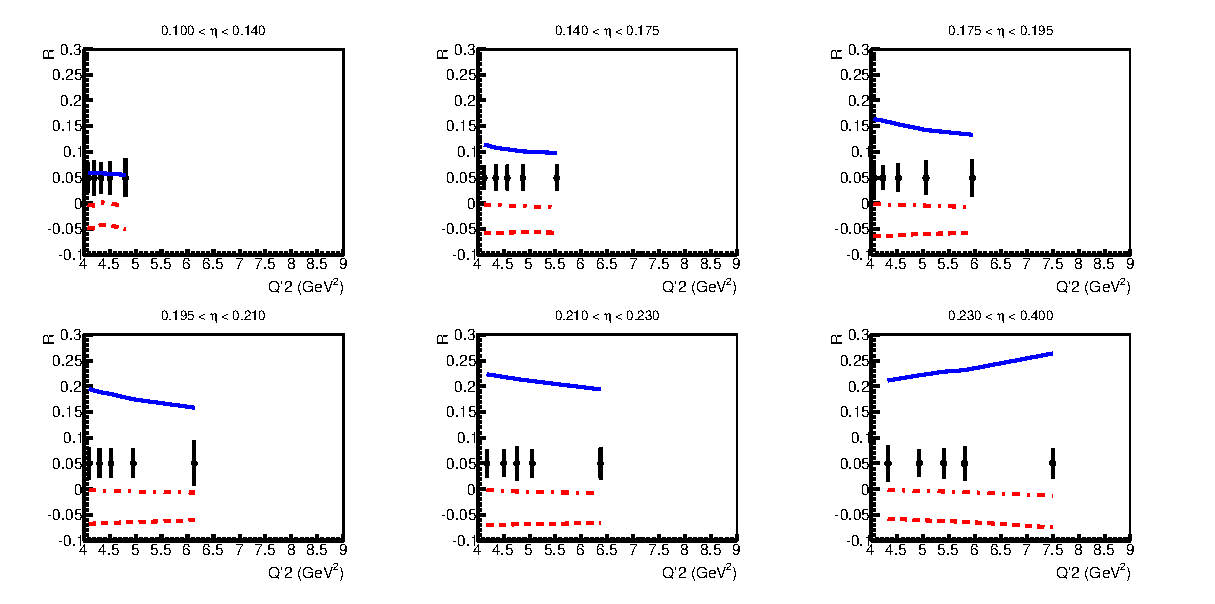
\includegraphics[scale=0.8]{R_etabin.eps}
\caption{\small{
The cosine moment of the weighted cross section, $R'$, shown as function of
$Q^{\prime 2}$ for six bins in $\eta$, in 0.2 GeV$^2$ wide bins in $|t|$
close to $t=t_{min}$. The curves correspond to leading-order, leading-twist 
calculations using two GPD models, the dual parametrization
\cite{Polyakov:2002wz,Guzey:2006xi,Guzey:2008ys,Polyakov:2008aa} (top, solid
blue curve) and the double distribution \cite{Radyushkin:1998es} with $D$-term
(middle, dash-dotted red curve) and without $D$-term (bottom, dashed red
curve). The error bars on the points correspond to 50 days of running.
The points are arbitrarily placed at $R' = 0.05$.}}
\label{fig:R_etabin}
\end{figure}

The same LO calculations can be applied to the $\eta$-dependence. The result
is shown in Fig.~\ref{fig:R_Q2bin}, where we see $R'$ as function of $\eta$
for two bins in $Q^{\prime 2}$, in 0.2 GeV$^2$ wide bins in $|t|$ close to 
$t=t_{min}$. The relation between $|t|$ and $\eta$ coverage can be seen in
Fig.~\ref{fig:t_eta_Q2bin}. As in Fig.~\ref{fig:R_etabin}, the top curve
(solid blue line) corresponds to the dual parametrization, and the middle
(dash-dotted red line) and lower (dashed red line) curves to the
double distribution with and without $D$-term, respectively. Here, the large
difference between the two models reflects the assumed dependencies of the
real part of GPD $H$ on $\tau$ (the equivalent of Bjorken $x$) that are shown
in Fig.~\ref{fig:ReImH_tau}, and to which the cosine moment $R'$ is sensitive.

\begin{figure}[t]
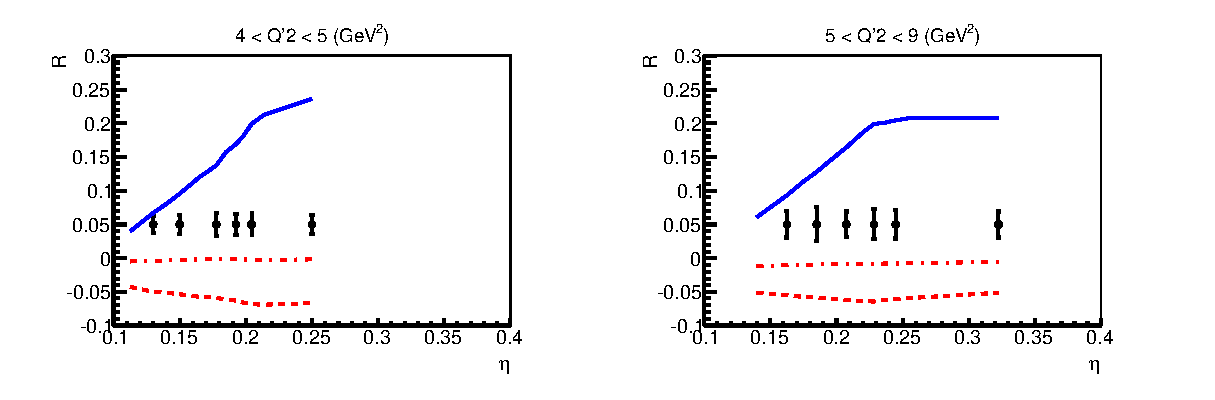
\includegraphics[scale=0.7]{R_Q2bin.eps}
\caption{\small{
The cosine moment of the weighted cross section, $R'$, shown as function of
$\eta$ for two bins in $Q^{\prime 2}$, in 0.2 GeV$^2$ wide bins in $|t|$
close to $t=t_{min}$. The curves correspond to leading-order, leading-twist
calculations using two GPD models, the dual parametrization 
\cite{Polyakov:2002wz,Guzey:2006xi,Guzey:2008ys,Polyakov:2008aa} (top, solid
blue curve) and the double distribution \cite{Radyushkin:1998es} with $D$-term
(middle, dash-dotted red curve) and without $D$-term (bottom, dashed red
curve). The error bars on the points correspond to 50 days of running.
The points are arbitrarily placed at $R' = 0.05$.}}
\label{fig:R_Q2bin}
\end{figure}

Fig.~\ref{fig:R_NLO} shows the projections based on the NLO calculations
described in Sect.~\ref{subsec:NLO}. Since the calculations in the figure
were made for $Q^{\prime 2} = 4$ GeV$^2$, the results are only shown for
one, bin in $Q^{\prime 2}$ between 4 and 6 GeV$^2$. Here, each point
corresponds to a 0.3 GeV$^2$ wide bin in $|t|$. 
The calculation was done using two GPD models: Goloskokov-Kroll (GK)
\cite{Goloskokov:2005sd,Goloskokov:2006hr,Goloskokov:2007nt,Kroll:2012sm}
and MSTW, a simple factorizing ansatz for the $t$-dependence
\cite{Berger:2001xd} with MSTW08 PDFs \cite{Martin:2009iq}.
Both LO and NLO results are shown. It is interesting to note that there is a
relatively model-independent trend in the calculations. The two upper curves
(dashed lines) are both NLO predictions, while the lower two (solid lines)
are the LO ones. It seems that for both models the NLO corrections shift
$R'$ towards more positive values, but the slope does not change much, and
hence the separation between the LO and NLO curves stays about the same for
all values of $\eta$ between 0.1 and 0.3 (going below $\eta$ of 0.1 the
separation in $R'$ does increase, but this is outside of JLab 12 GeV
kinematics). The GK model prediction (blue curves) for $R'$ is consistently
somewhat higher than MSTW (red curves) for both LO and NLO, but this
difference is small compared with the overall shift due to the NLO
corrections.
The model-independence mirrors the discussion in Sect.~\ref{subsec:NLO} where,
for instance, Fig.~\ref{fig:TCSRe2x2} suggests that the general features of
the NLO calculations do not strongly depend on the choice of model. That said,
it is worth keeping in mind that the GK model is based on $\tilde{H}$ and $H$,
while MSTW only incorporates $H$, so the predictions shown assume that other
contributions are small. It is hoped that $Q^{\prime 2}$ evolution will
be incorporated into the NLO calculation in the near future, which would
allow for reliable projections also at higher values of $Q^{\prime 2}$.

\begin{figure}[t]
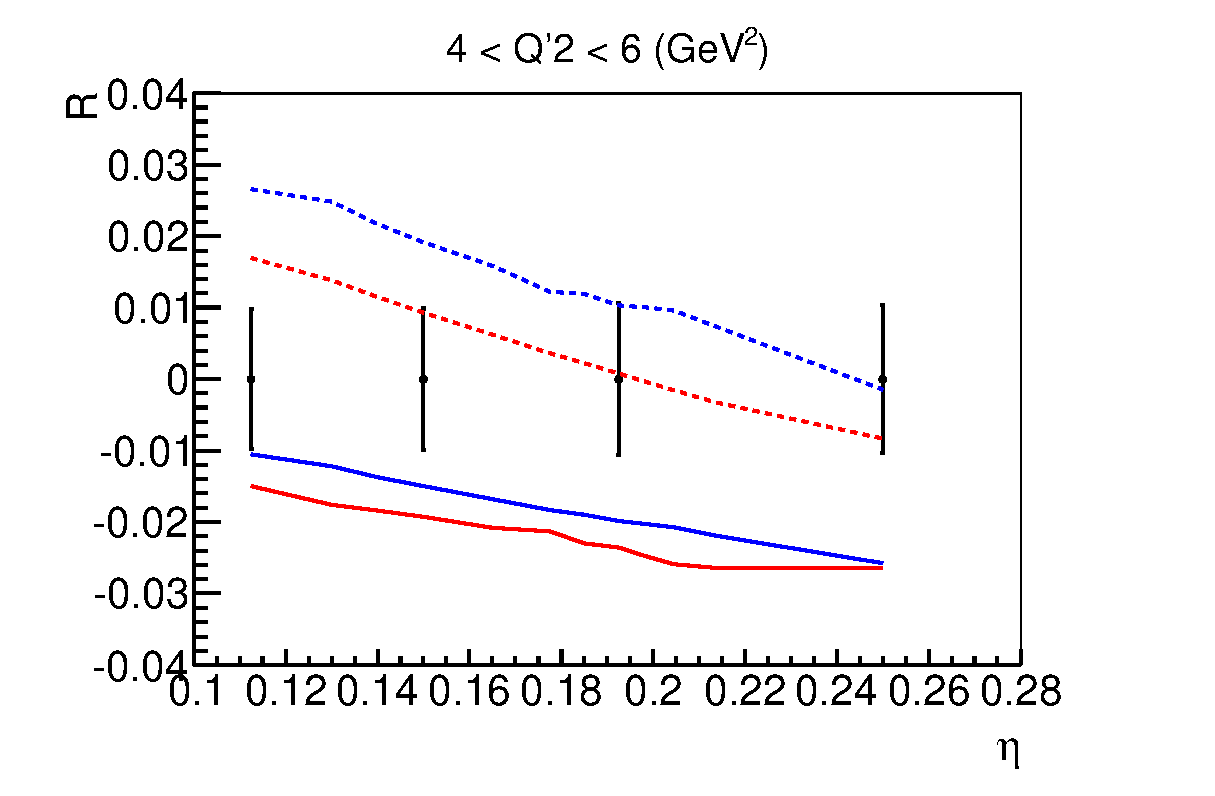
\includegraphics[scale=0.45]{R_NLO.eps}
\caption{\small{
The cosine moment of the weighted cross section, $R'$, shown as function
of $\eta$ for in a bin of $Q^{\prime 2}$ from 4 to 6 GeV$^2$ and a 0.3
GeV$^2$ wide bin of $|t|$. The upper (dotted) curves are the NLO predictions,
while the (solid) lower pair are the LO ones. Within each pair, the upper
(blue) curve was calculated using the GK model and the lower (red) one using
MSTW. The error bars on the points correspond to 50 days of running.
The points are arbitrarily placed at $R' = 0$.}}
\label{fig:R_NLO}
\end{figure}

In conclusion, the physics of deeply-virtual Compton scattering is a rich
topic, and the possibility to study the universality of GPDs and the
timelike-spacelike correspondence through TCS will add an important piece to
the puzzle. This proposed high-luminosity measurement in SoLID will make it
possible to study  the $Q^{\prime 2}$-dependence and the $\eta$-dependence.
The former will allow us to establish the scaling properties expected for
factorization, and the magnitude of our benchmark observable $R'$ will, as
shown in Fig.~\ref{fig:R_etabin}, also provide some guidance on GPD modeling.

Once the $Q^{\prime 2}$-dependence is understood, the data can be binned in
much wider bins of $Q^{\prime 2}$ for the measurement of the
$\eta$-dependence. Here, a comparison of the LO calculations for
our benchmark observable $R'$, shown in Fig.~\ref{fig:R_Q2bin}, indicates
that our sensitivity will allow us to determine whether there is a strong
$\eta$-dependence in the real part of GPD $H$ as assumed in the dual
parametrization, or if it is relatively flat as shown for the double
distribution. This alone would be a very important contribution to our
understanding of the behavior of GPDs. It is also interesting to note that LO
calculations using both the GK and MSTW models shown in Fig.~\ref{fig:R_NLO}
exhibit an $\eta$-dependence, but with a smaller and opposite slope to
that of the dual parametrization.

Measuring the $\eta$-dependence is also important for studying NLO effects.
However, in this respect it is interesting to note that our benchmark
observable $R'$ provides us with a more limited sensitivity to the NLO
corrections that one might think based on, for instance,
Fig.~\ref{fig:TCSRe2x2}. For $R'$, NLO effects create a clear shift towards
higher values, but the impact on the slope seems to be modest over the range
of $\eta$ relevant for JLab 12 GeV.
Since the NLO corrections are predominantly due to gluons, and little is
known about the gluon GPD, this scenario seems very encouraging. On one hand
it suggests that one could constrain the NLO gluonic contributions through
the magnitude of $R'$, but one the other that this would still be a good
observable for studying the behavior of quark GPDs, such as the
$\eta$-dependence of the real part of GPD $H$, even at the lower
end of the accessible $\eta$ range.
Of course, it would be even more interesting if it turned out that there were
other observables that were more sensitive to the gluons than $R'$. Then the
the lower part of the $\eta$ range covered by this proposed TCS experiment
could, perhaps in conjunction with vector meson production, provide a novel
approach for probing the glue in the valence region.
